\subsection{Le trajectographe}\label{chapter-LHC-section-CMS-subsec-tracker}
Le trajectographe couvre la partie centrale du détecteur, son acceptation correspondant à la région $\abs{\eta} < \num{2.5}$.
Les particules chargées laissent des signaux de leur passage dans les différents modules du trajectographe en les traversant.
Il est ainsi essentiel à la reconstruction des vertex des événements du LHC.
Les particules chargées se trouvant hors de son acceptation mais visibles dans d'autres sous-détecteurs sont reconstruites comme des particules neutres.
\par Deux types de modules composent le trajectographe de CMS~\cite{cms_paper,CERN-LHCC-98-006,CMS-TDR-11,CMS-TRK-11-001,CMS-TRK-17-001}.
Dans sa partie interne, \ie\ la plus centrale en rayon, des modules à pixels de silicium sont utilisés.
Au début du Run~II du LHC, le \CMSbarrel\ du trajectographe interne était composé de trois couches de pixels à \num{4.4}, \num{7.3} et \SI{10.2}{\centi\meter} de rayon~\cite{cms_paper} et les \CMSendcaps\ de deux disques de pixels.
Le trajectographe interne est visible en rouge sur la figure~\ref{fig-CMS-trk_detailed_scheme}.
Les pixels ont une surface de $\num{100}\times\SI{150}{\micro\meter^2}$.
La résolution spatiale de cette partie du trajectographe est de l'ordre de \SI{10}{\micro\meter}~\cite{cms_paper} et permet d'obtenir une bonne reconstruction des vertex.
En mars 2017, cette partie du trajectographe a été remplacée~\cite{CMS-TDR-11,cms_trk_upgrade_2017}.
Elle comporte à présent quatre couches de pixels dans la partie \CMSbarrel\ à \num{2.9}, \num{6.8}, \num{10.9} et \SI{16.0}{\centi\meter} de rayon.
Dans les \CMSendcaps, les disques ont également été repensés afin d'obtenir quatre points de passage pour les traces telles que $\abs{\eta}<\num{2.5}$.
Une comparaison des trajectographes à pixels utilisés en 2016 (Phase-0) et à partir de 2017 (Phase-1) est illustrée sur la figure~\ref{fig-chapter-LHC-section-CMS-subsec-tracker-2017-upgrade}.
Cette modification du détecteur permet d'améliorer la reconstruction des vertex ainsi que l'efficacité de l'identification de jets issus de quarks~\quarkb.
\par
De \num{20} à \SI{116}{\centi\meter} de rayon se trouve le trajectographe à piste, lui-même composé de trois sous-parties.
La première de ces sous-parties comporte un \CMSbarrel\ (TIB, \emph{Tracker Inner Barrel}) de quatre couches et trois disques (TID, \emph{Tracker Inner Disks}) vers l'avant.
Les pistes dans ces couches sont parallèles au faisceau dans le TIB et axiales dans les TID.
Elles permettent d'obtenir une résolution de \SI{23}{\micro\meter} et \SI{35}{\micro\meter} respectivement~\cite{cms_paper}.
Le TIB et les TID sont entourés par le \CMSbarrel\ du trajectographe externe (TOB, \emph{Tracker Outer Barrel}) de six couches.
Le TOB a une résolution de \SI{53}{\micro\meter} pour ses quatre premières couches et de \SI{35}{\micro\meter} ensuite~\cite{cms_paper}.
Enfin, les \CMSendcaps\ du trajectographe externe (TEC, \emph{Tracker EndCaps}) se situent aux extrémités du dispositif.
\par
Les trajectoires des particules chargées sont alors reconstruites par un ajustement aux différents points de passage dans le trajectographe.
À partir de ces trajectoires, il est possible de déterminer le signe de la charge électrique et l'impulsion transverse des particules à l'aide de l'équation~\eqref{eq-chapter-LHC-section-CMS-subsec-solenoide-rayon_courbure}.
Les résolutions obtenues sur les impulsions transverses des muons et des particules chargées à l'aide du trajectographe sont présentées sur la figure~\ref{fig-chapter-LHC-section-CMS-subsec-tracker-pT-resolution}.
\begin{figure}[h]
\centering
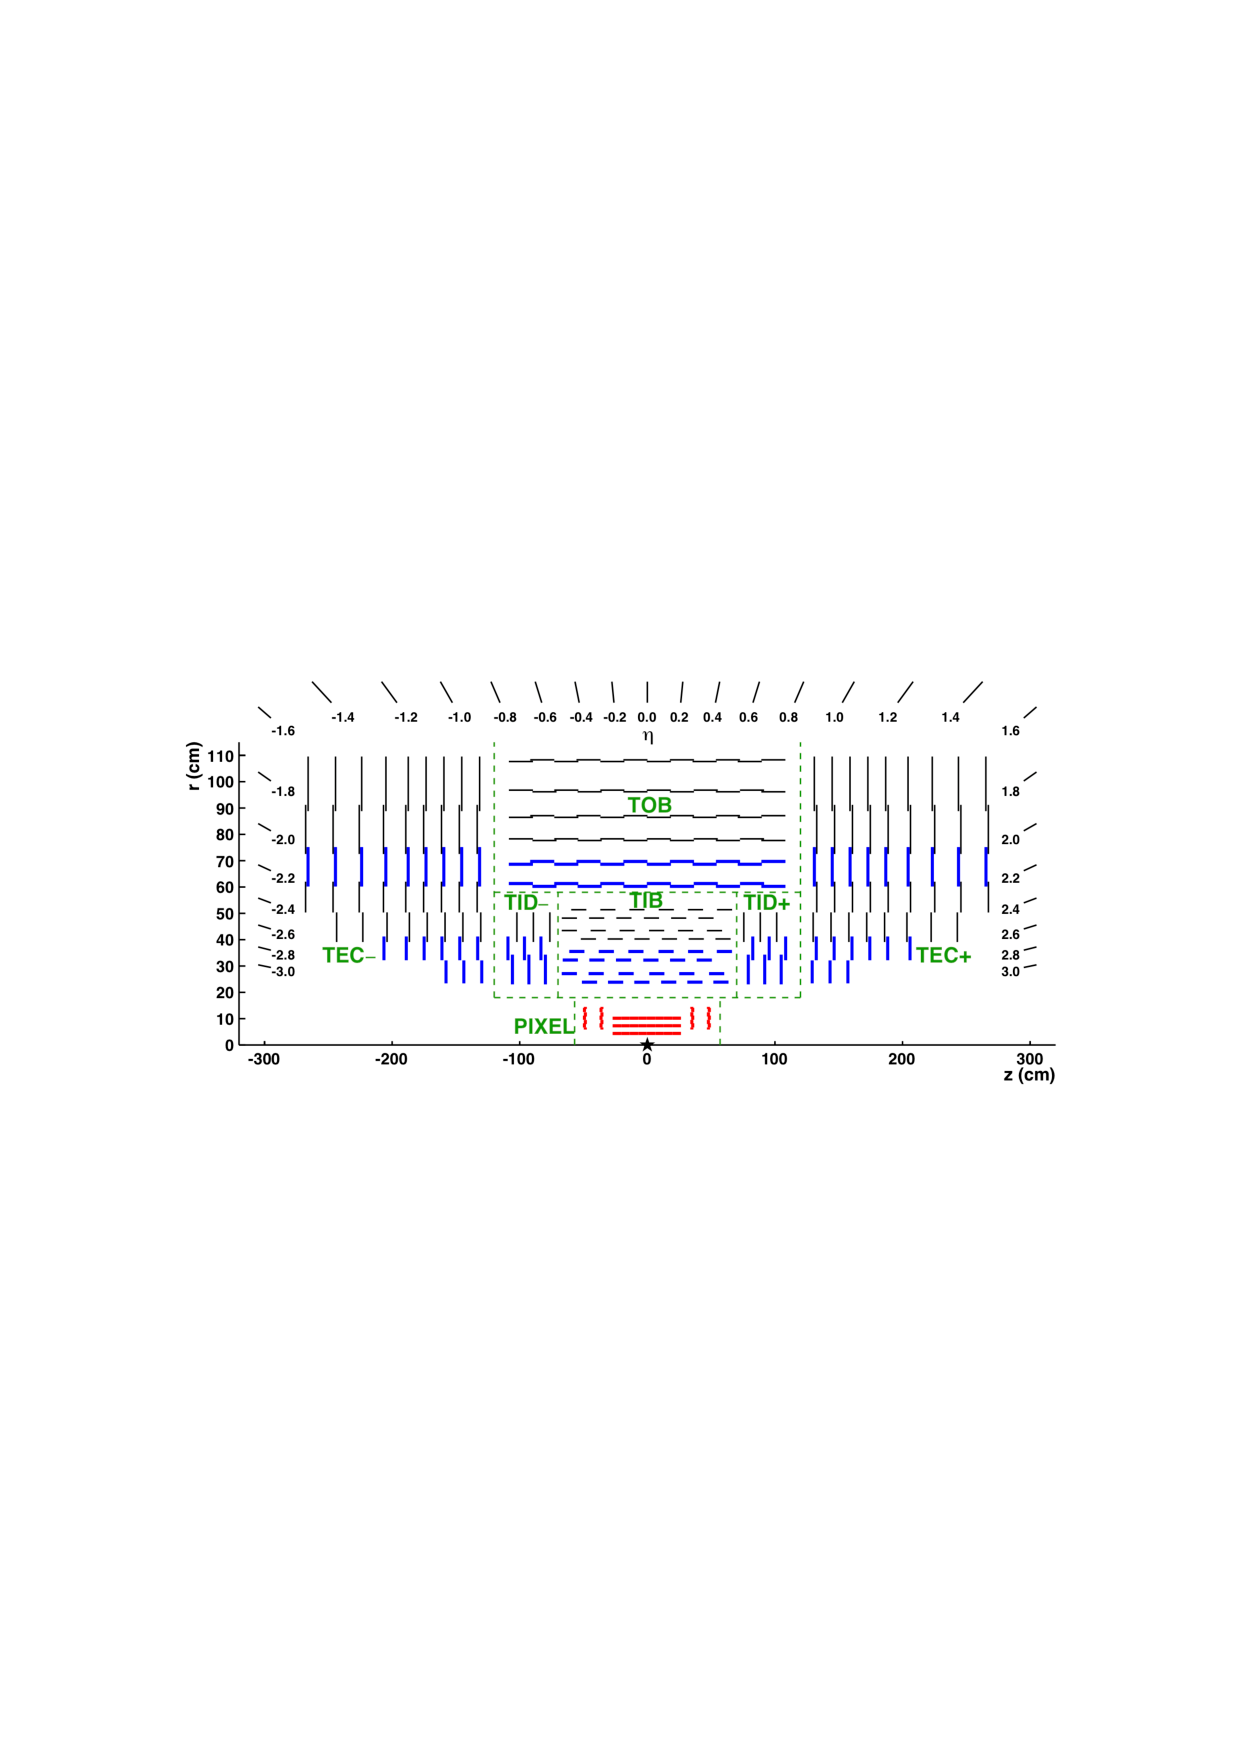
\includegraphics[width=\textwidth]{\PhDthesisdir/plots_and_images/from_CMS-TRK-17-001/CMS-TRK-17-001_Figure_001-a.pdf}
\caption[Schéma détaillé du trajectographe du détecteur CMS.]{Schéma détaillé du trajectographe du détecteur CMS dans le plan \plane{r}{z}~\cite{CMS-TRK-11-001,CMS-TRK-17-001}. Le trajectographe est symétrique par rapport à l'axe \axis{z}, axe du faisceau. Le centre du trajectographe, correspondant approximativement au lieu des collisions, est indiqué par une étoile. Les différentes sous-parties du trajectographe sont délimitées par les pointillés verts. Les modules à piste donnant des signaux en deux dimensions sont indiqués en lignes noires fines et ceux donnant des signaux en trois dimensions en lignes bleues épaisses. Ces derniers sont en fait constitués de deux modules à piste dos à dos dont l'un est tourné de \ang{90}. Les modules à pixels, en rouge, permettent également d'obtenir des signaux à trois dimensions. Les légers décalages des modules leur permettent d'éviter tout angle mort dans la zone d'acceptation du détecteur.}
\label{fig-CMS-trk_detailed_scheme}
\end{figure}
\begin{figure}[h]
\centering
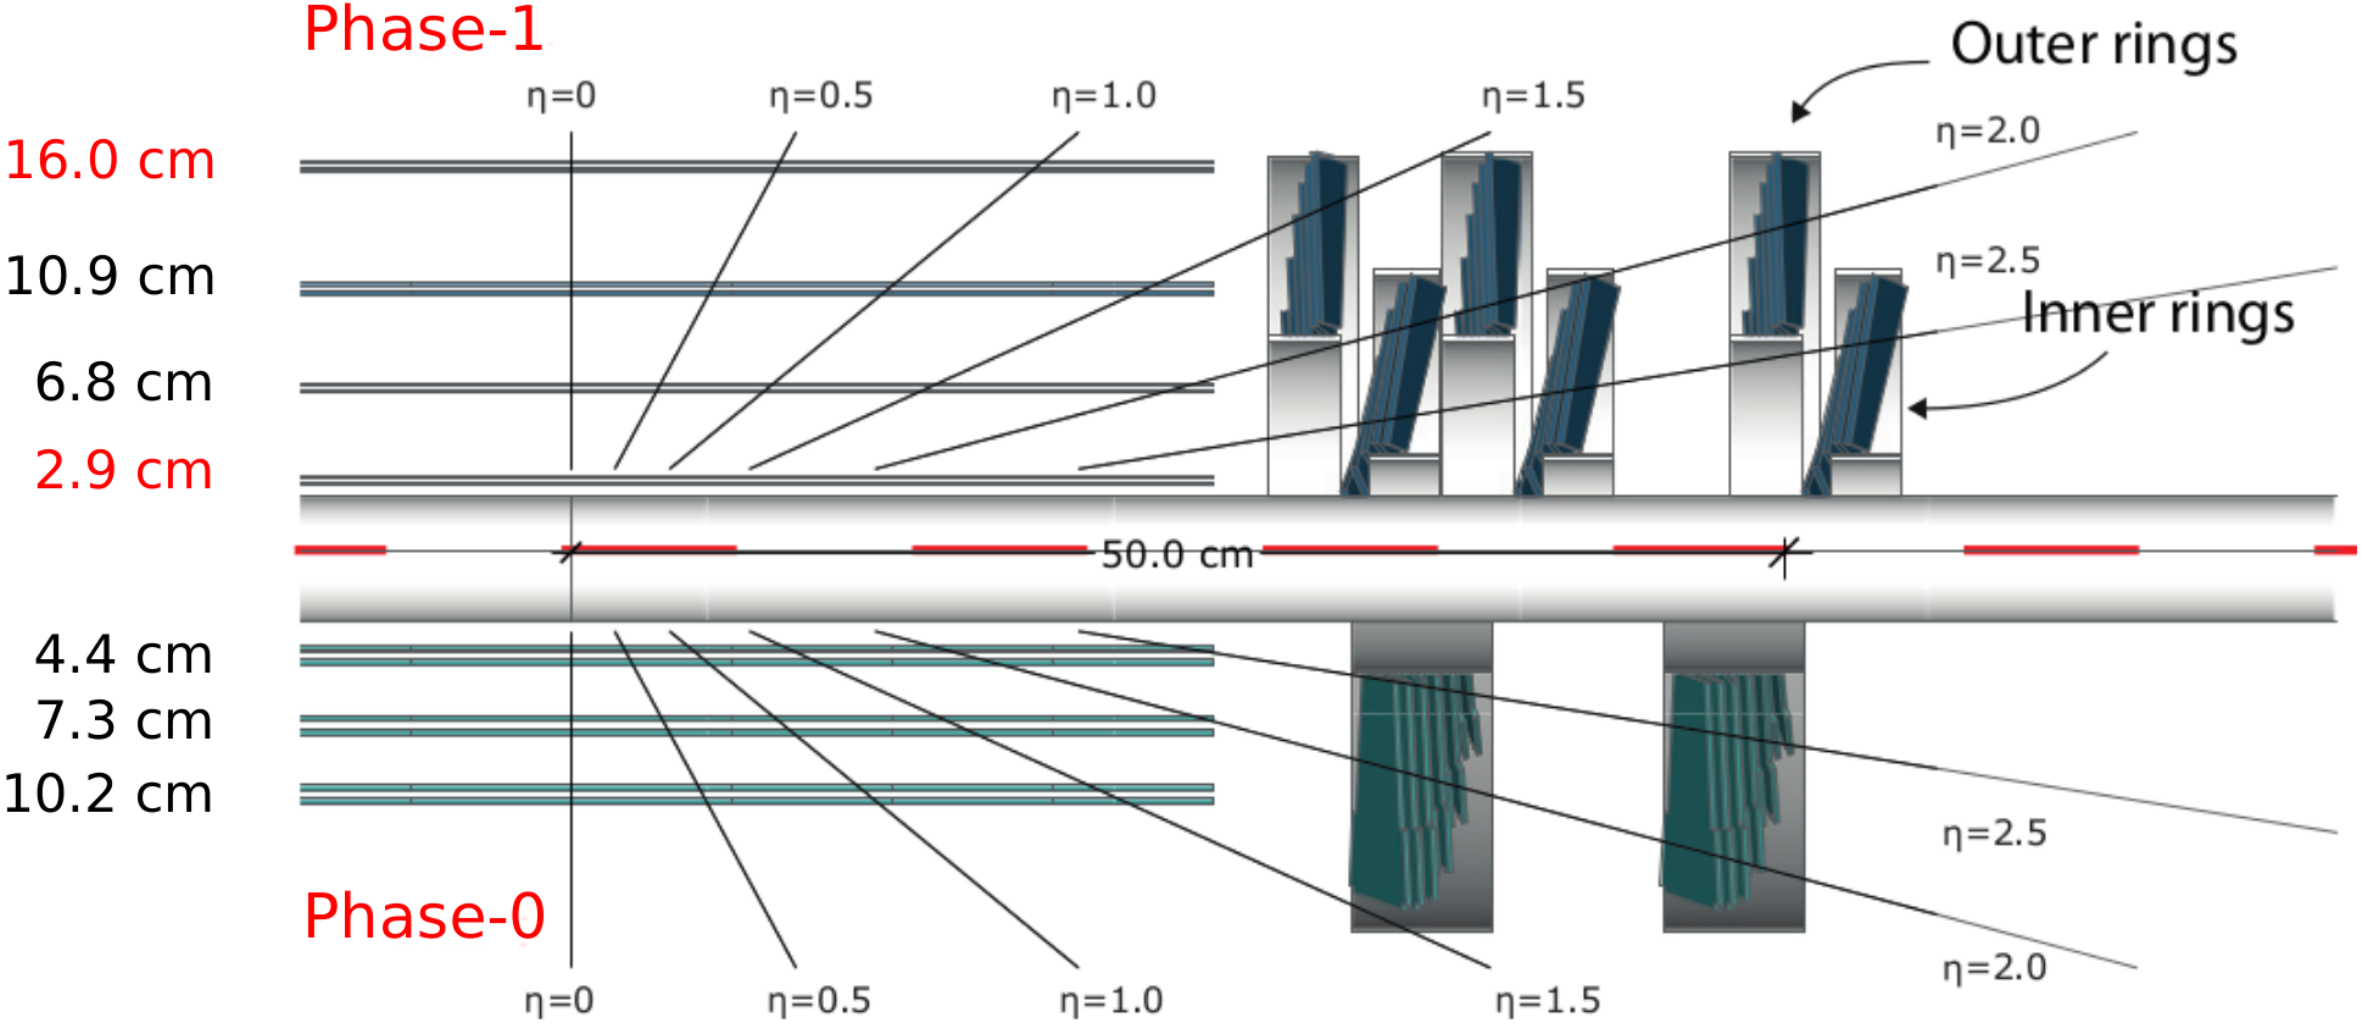
\includegraphics[width=0.9\linewidth]{\PhDthesisdir/plots_and_images/from_cms_trk_upgrade_2017/fig2.png}
\caption[Comparaison des trajectographes à pixels utilisés en 2016 et à partir de 2017.]{Comparaison des trajectographes à pixels utilisés en 2016 (Phase-0, en bas) et à partir de 2017 (Phase-1, en haut) \cite{CMS-TDR-11,cms_trk_upgrade_2017}.}
\label{fig-chapter-LHC-section-CMS-subsec-tracker-2017-upgrade}
\end{figure}
\begin{figure}[h]
\centering
\subcaptionbox{Résolution pour des muons seuls et isolés.\label{subfig-chapter-LHC-section-CMS-subsec-tracker-pT-resolution-muons}}[.45\textwidth]
{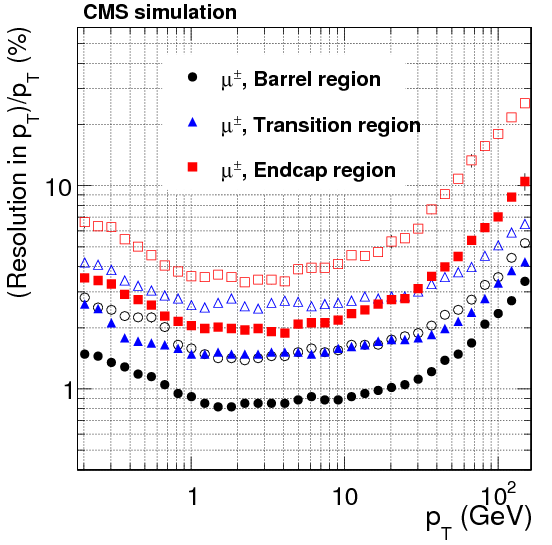
\includegraphics[width=.45\textwidth]{\PhDthesisdir/plots_and_images/from_CMS-TRK-11-001/figs_2011_trackPerformance_MC_SingleParticles_mu_resolutionPtVsPt.png}}
\hfill
\subcaptionbox{Résolution pour des particules chargées.\label{subfig-chapter-LHC-section-CMS-subsec-tracker-pT-resolution-charged_ptcs}}[.45\textwidth]
{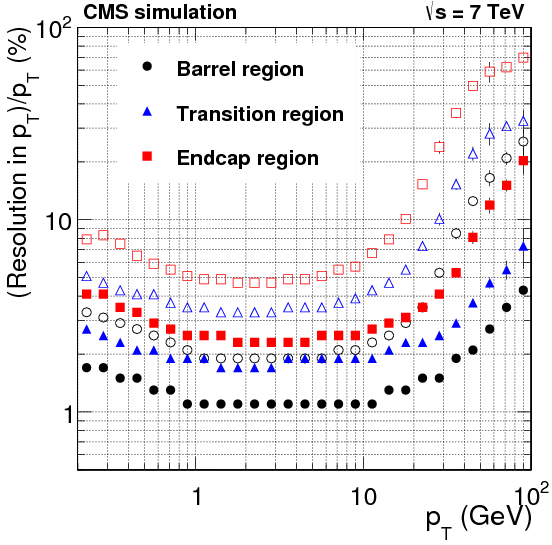
\includegraphics[width=.45\textwidth]{\PhDthesisdir/plots_and_images/from_CMS-TRK-11-001/figs_2011_trackPerformance_MC_ttbarHpWithPuSplitByEta_resolutionPtVsPt.png}}
\caption[Résolution en \pT\ du trajectographe.]{Résolution en \pT, en fonction de \pT, du trajectographe pour différentes particules~\cite{CMS-TRK-11-001}. Les symboles pleins correspondent à la demi-largeur à \SI{68}{\%} de la distribution, les symboles creux à \SI{90}{\%}.}
\label{fig-chapter-LHC-section-CMS-subsec-tracker-pT-resolution}
\end{figure}
